\chapter{RSA (Rivest-Shamir-Adleman)}
\section{Generazione delle chiavi}
La creazione della coppia di chiavi spetta al destinatario.
\begin{enumerate}
    \item Si scelgono due numeri interi e primi $p$, $q$ molto grandi ($\approx 1000$ bit) (adesso si consiglia che $p \cdot q \approx 2048$ bit per avere una protezione fino al 2030, mentre per una protezione di maggiore durata si consigliano 3072 bit). Ovviamente questo passo deve essere fatto in tempo polinomiale (la generazione di $p$ e $q$): si generano sequenze casuali (nei modi già visti) e \textbf{\underline{si testa la primalità utilizzando il test di Miller-Rabin}}.
    \item Si calcola il prodotto $n$ e la funzione di Eulero $\phi(n)$ (questo è facile da calcolare, poichè conosciamo la scomposizione di $n$, si ricordi la formula vista indietro)
    \begin{align*}
    	n&=p\cdot q\\
    	\phi(n)&=(p-1) \cdot (q-1)
   \end{align*}Anche qui operazioni in tempo polinomiale nella grandezza dell'input.
    \item Si sceglie $e < \phi(n)$ tale che $e$ e $\phi(n)$ siano coprimi
    $$\text{MCD}(e, \phi(n))=1$$
    \item Si calcola $$d = e^{-1} \text{ mod } \phi(n)$$ Anche questo si può calcolare in tempo polinomiale usando l'algoritmo di Euclide esteso. Si osservi che essendo $MCD(e, \phi(n))=1$ si ha unicità della soluzione ($e^{-1}$).
\end{enumerate}

\paragraph{Risultato finale} Alla fine si hanno quindi le due chiavi:
\begin{align*}
K_{pub} = <e,n> && K_{priv} = <d,n>
\end{align*}
Naturalmente va tenuto segreto anche il resto delle informazioni: $p$, $q$, $\phi(n)$.

\section{Cifratura e decifratura}
\[\boxed{\text{I messaggi sono sequenze binarie trattate come interi!}}\]
\begin{itemize}
	\item  \textbf{NB}. Indichiamo il messaggio $m$ e imponiamo $m<n$. In caso contrario potrebbero emergere ambiguità nella decifrazioni: la cosa è chiara nella dimostrazione di correttezza, non sarà possibile arrivare a conclusione senza adottare questa condizione. Se $m \geq n$ allora dividiamo il messaggio $m$ in blocchi di $b = \lfloor \log_2n \rfloor$ bit (sempre con la stessa chiave) e cifriamo ciascuno (eventualmente con CBC).
	\item \textbf{NB2}. Solitamente si fissa un limite inferiore comune per la dimensione dei blocchi, prevenendo così l'uso di cifrari poco sicuri. Supponiamo che il blocco sia di almeno $b$ bit: i messaggi saranno numeri fino a $2^b$, ma lo stesso massimo deve essere minore di $n$ per la condizione detta $$m < 2^b < n$$ 
	\item \textbf{Cifratura}. Abbiamo la chiave pubblica $<e,n>$ e il messaggio $m$
	$$ c = C(m, K_{pub}) = m^{e} \text{ mod } n$$
	con $m<n, c <n$
	\item \textbf{Decifrazione}. Abbiamo la chiave privata $<d,n>$ e il crittogramma $c$
	$$ m = D(c, K_{priv}) = c^{d} \text{ mod } n$$
\end{itemize} 
Sicuramente il cifrario RSA è molto elegante! L'utilizzo del modulo garantisce la sicurezza del cifrario. 

\subsection{Esempio}
Consideriamo il seguente esempio.
\begin{enumerate}
	\item Calcoliamo $p,q$ e la funzione di Eulero
	\begin{align*}
		p=5, q= 11 \Longrightarrow \,&n = p \cdot q = 5 \cdot 11 = 55\\
		&\phi(n)=(p-1)\cdot(q-1)=40
	\end{align*}
	\item Scegliamo un valore $e$ coprimo con $40$: prendiamo $e=7$, che è coprimo con $\phi(n)=40$ poichè
	$$\text{MCD}(7,40)=1$$
	\item Applichiamo l'algoritmo di Euclide esteso per calcolare l'inverso moltiplicativo\\$d=7^{-1}\text{ mod }40$
	\begin{verbatim}
	EE(7,40) ---> <1, -17>
	EE(40, 7 mod 40) = EE(40, 7) ---> <1,3,-2 - floor(40/7)*3 = <1,3,-17>
	EE(7, 40 mod 7) = EE(7, 5) ---> <1, -2, 1 - floor(7/5)*(-2)> = <1,-2,+3>
	EE(5, 7 mod 5) = EE(5, 2) ---> <1,1,0 - floor(5/2)*1> = <1,1,-2>
	EE(2, 5 mod 2) = EE(2, 1) ---> <1,0, 1 -  floor(2/1)*0> = <1,0,1>
	EE(1, 0) ---> <1,1,0>
	\end{verbatim}
	L'inverso risultante è $-17$, che è negativo: visto che lavoriamo in modulo $40$ sommiamo $40$. Morale della favola:
	$$d=-17 \text{ mod } 40 = 23 \text{ mod } 40=23$$
	\item Abbiamo ottenuto 
	\begin{align*}
		K_{pub}=<7,55>&&K_{priv}=<23, 55>
	\end{align*}
	Per decifrare faremo ($m< 55$)
	\begin{align*}
		c&=m^7 \text{ mod }55\\m&=c^{23} \text{ mod } 55
	\end{align*}
	Si possono eseguire i calcoli in tempo polinomiale tramite l'algoritmo delle quadrature successive.
\end{enumerate}


\section{Dimostrazione del teorema di correttezza del cifrario}
Dimostrare la correttezza del cifrario significa dimostrare che
$$ D(C(m, K_{pub}), K_{priv}) = m $$
nel contesto del RSA significa dimostrare che ($\forall  m < n$)
$$c^d\text{ mod }n=(m^e \text{ mod } n)^d \text{ mod } n = \boxed{m^{ed} \text{ mod } n = m}$$
%diciamo questo dalla nuova proprietà dell'operatore modulo introdotta qualche pagina fa
%$$a^{r \times s} \text{ mod } m &= (a^r \text{ mod } m)^{s} \text{ mod } m$$
La cosa non è così ovvia: $e$ e $d$ sono l'uno l'inverso dell'altro ma rispetto a mod $\phi(n)$ e non mod $n$ (\textbf{\underline{ricordare come abbiamo generato la chiave}})
$$ed \equiv 1 \text{ mod } \phi(n)$$
La dimostrazione del teorema di correttezza del cifrario si fa affrontando tre casi. Si prenda il prodotto $n=p\cdot q$ e chiediamoci: cosa succede se provo a dividere il messaggio $m$ (che trattiamo come intero) per $q$? Cosa succede se faccio lo stesso con $p$?

\subsection{Caso: il messaggio $m$ è divisibile sia per $q$ che per $p$}
Avere $m$ divisibile sia per $p$ che per $q$ significa che è divisibile per $n$. 
\[\boxed{\text{Ciò non è possibile perché abbiamo imposto $m < n$.}}\]
La divisione risulta possibile solo se $m$ è almeno uguale ad $n$ (e quindi se $m \geq n$).
$\hfill\blacksquare$

\subsection{Caso: $p$ e $q$ non dividono il messaggio $m$}
Se $p$ e $q$ non dividono $m$ allora $m$ ed $n$ sono coprimi, cioè: $\text{MCD}(m,n)=1$. Riprendiamo le seguenti cose.
\begin{itemize}
	\item \textbf{Teorema di Eulero}: $m^{\phi(n)} \equiv 1 \text{ mod }n$ (possiamo dirlo visto che $\text{MCD}(m,n)=1$)
	\item \textbf{Definizione di inverso} (con $r \in \mathbb{N}$): $ed \equiv 1 \text{ mod } \phi(n) \Longrightarrow ed=1+r \cdot \phi(n)$
\end{itemize}
Partendo da quest'ultima cosa scriviamo
$$ m^{ed} \text{ mod } n = m^{1 + r \cdot \phi(n)} \text{ mod } n = m \cdot (m^{\phi(n)})^{r} \text{ mod } n$$
Abbiamo detto che $m$ ed $n$ sono coprimi, \textbf{\underline{quindi possiamo utilizzare il teorema di Eulero}}. 
$$ m \cdot 1^r \text{ mod } n = m \text{ mod } n = m $$
L'ultimo passaggio è certo (la rimozione del modulo) poichè $m <n$
$\hfill\blacksquare$
\subsection{Caso: il messaggio $m$ è divisibile per $p$ e non per $q$ (o viceversa)}
Supponiamo che $m$ e $n$ non siano coprimi: in particolare abbiamo $m$ divisibile per $p$ e non per $q$ (o viceversa). Non possiamo usare il teorema di Eulero come appena fatto! 
\paragraph{Numero  divisibile }Se $p$ è multiplo di $m$ allora
$$m \equiv 0 \text{ mod }p \longrightarrow m \text{ mod }p=0$$
tutte le potenze di $m$ continueranno ad essere divisibili per $p$, quindi
$$\forall r \in \mathbb{N}\,\,\,\,\, \,\,\,m^r\equiv 0 \text{ mod }p \longrightarrow m^r  \text{ mod } p=0$$
siccome sia $m^r$ che $m$ sono congrui a $0$ modulo $p$ allora lo è pure la differenza
$$\forall r \in \mathbb{N}\,\,\,\,\,\,\,\,m^r-m\equiv 0 \text{ mod } p \longrightarrow (m^r-m) \text{ mod } p = 0$$
Possiamo porre $r=ed$
$$m^{ed}-m\equiv 0 \text{ mod } p$$
\paragraph{Numero non divisibile} Ricaviamo una relazione simile anche per $q$. Sappiamo che $q$ ed $m$ sono coprimi, dunque è applicabile il teorema di Eulero
$$m^{\phi(q)} \equiv 1 \text{ mod }q \longrightarrow m^{\phi(q)} \text{ mod } q = 1$$
Facciamo i seguenti calcoli:
\begin{align*}
	m^{ed} \text{ mod } q = m^{\phi(n) \cdot r + 1} \text{ mod } q &= m \cdot m^{r(p-1)\cdot(q-1)} \text{ mod }q=m \cdot (m^{(q-1)})^{(p-1)\cdot{r}} \text{ mod } q=\\&=m \cdot (m^{\phi(q)})^{(p-1)\cdot{r}} \text{ mod } q=m \text{ mod } q\end{align*}
$q$ è numero primo, dunque la funzione di Eulero è il numero decrementato ($\phi(q)=q-1$).  Concludiamo:
$$ m^{ed} \equiv m \text{ mod } q \implies m^{ed} - m \equiv 0 \text{ mod } q $$
\paragraph{Conclusione} Abbiamo quindi ottenuto:
\[
    \begin{cases}
    $$ m^{ed} - m \equiv 0 \text{ mod } q $$ \\ 
    $$ m^{ed} - m \equiv 0 \text{ mod } p $$
    \end{cases}
\]
che significa che $ m^{ed} -m $ è divisibile sia per $p$ che per $q$ quindi lo sarà anche per $n = p \cdot q$, possiamo quindi dire:
$$ m^{ed} -m \equiv 0 \text{ mod } n \Longrightarrow m^{ed} \equiv m \text{ mod } n = m $$
L'ultimo passaggio è certo (la rimozione del modulo) poichè $m <n$
$\hfill\blacksquare$

\section{Sicurezza del cifrario ed attacchi}
\subsection{Soluzioni equivalenti alla fattorizzazione}
La sicurezza è legata alla difficoltà della fattorizzazione di un numero molto grande. 
\[\boxed{\text{La fattorizzazione è C.S. (non si sa se  C.N.) per rompere RSA in tempo polinomiale}}\]
Se fattorizzo $n$ trovo $p$ e $q$, e quindi $\phi(n)=(p-1)(q-1)$. 
Consideriamo le possibili alternative, tutte equivalenti alla fattorizzazione.
\begin{itemize}
	\item \textbf{Calcolo della radice in modulo}. 
	$$m = \sqrt[e]{c} \mod n$$
	Il calcolo è difficile \textbf{\underline{almeno}} quanto la fattorizzazione di $n$ ($n$ composto), non emerge utilità nello svolgere questi calcoli.
	\item \textbf{Calcolo di $\phi(n)$ direttamente da $n$}.
	
	Il calcolo di $\phi(n)$ a partire da $n$ è computazionalmente equivalente alla fattorizzazione di $n$: se io calcolo $\phi(n)$ da $n$ allora conoscendo i due posso trovare $p$ e $q$ in tempo polinomiale. 
	$$\boxed{n = p \cdot q \xrightarrow{} \phi(n) = (p-1) \cdot (q-1)}$$
	Calcoliamo $\phi(n)$
	\begin{align*}
		\phi(n) &= (p-1) \cdot (q-1)= p \cdot q - (p+q) + 1 = n - (p+q) + 1
	\end{align*}
	ottengo $ x_1 = p+q = n - \phi(n) + 1 $, 	poi $ (p-q)^2 = (p+q)^2 - 4 \cdot n = (x_1)^2 - 4 \cdot n $
	
	quindi $ x_2 = p - q = \sqrt{x_1^{2} - 4 \cdot n}$
	
	ottengo che i due problemi sono equivalenti.
	\[
	\begin{cases}
		x_1 = p + q \\ 
		x_2 = p - q
	\end{cases}	\Longrightarrow \begin{cases}
		p = \frac{x_1 + x_2}{2} \\
		q = \frac{x_1 - x_2}{2}
	\end{cases}
	\]
	
	\item \textbf{Attacco esauriente su $d$}. 
	
	Un altro attacco che posso fare è cercare di brutare $d$ partendo da $(n,e)$.
\end{itemize}
\paragraph{NB} Fattorizzare non è \emph{NP-hard} quindi non si esclude che esista un algoritmo efficiente.
\pagebreak 

\subsection{Osservazioni sulla fattorizzazione di n}
La fattorizzazione è difficile, ma non più come una volta: l'hardware migliora e gli algoritmi si affinano (pur rimanendo costosi sul piano computazionale). Non è definito un limite inferiore: questo significa che in futuro potrebbero emergere algoritmi aventi migliore complessità.
\begin{itemize}
    \item Esistono algoritmi di \textbf{complessità sub-esponenziale} come il \emph{General Number Field Sieve} (GNFS) che richiede O($2^{\sqrt{b \cdot \log b}}$) con $b$ la dimensione di $n$ (un attacco brute-force è O($2^b$)).
    \item Con la potenza di calcolo attuale usando GNFS si fattorizza fino a 768 bit. Nuovi algoritmi hanno ridotto il numero di bit di sicurezza, ergo hanno comportato un aumento del numero di bit necessari per garantire la sicurezza. Per avere una sicurezza come quella che si ottiene con AES a 128 bit si dovrebbe ricorrere a $n$ con circa 3072 bit, si sale addirittura a 15360 bit di modulo se lo si compara con AES256.
    \begin{center}
    	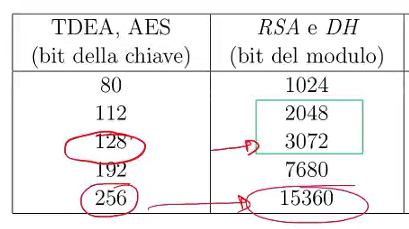
\includegraphics[scale=.8]{images/25.PNG}
    \end{center}
    Nell'AES i bit della chiave sono tutti bit di sicurezza, mentre nel RSA i bit del modulo non sono tutti di sicurezza: \textbf{si hanno attacchi più efficienti del forza bruta} (motivo per cui nel tempo i bit aumentano).
\end{itemize}

\subsection{Scelta ottimale dei valori $p,q$}
I numeri $p$ e $q$ vanno scelti \emph{molto} grandi, \emph{entrambi} attorno ai 1700 bit: se uno è troppo piccolo la fattorizzazione ci mette poco a individuare il numero piccolo.
\begin{itemize}
	\item Sia $p-1$ che $q-1$ devono contenere fattori grandi (altrimenti $n$ si fattorizza velocemente).
	\item $\text{MCD}(p-1, q-1)$ deve essere piccolo! Conviene scegliere $p$ e $q$ tali che i numeri $\frac{p-1}{2}$ e $\frac{q-1}{2}$ siano coprimi.
	\item \textbf{Norma di buon senso: cambiare sempre entrambi i numeri primi}.
	
	Mai riutilizzare uno dei primi per altri moduli: il crittoanalista potrebbe pensare che io per pigrizia ho generato un nuovo numero primo mantenendo l'altro numero primo. La cosa non è un problema, sappiamo ottenere i numeri primi in tempo polinomiale.
	\[\begin{cases}
			n_1 = p \cdot q_1 \\
			n_2 = p \cdot q_2
		\end{cases}
		\implies \text{MCD}(n_1, n_2) = p
	\]

\item \textbf{Attacco con $p$ e $q$ simili}.

Scegliere $p$ e $q$ distanti tra loro! Se $p \approx q$ allora si ha un attacco molto efficiente dove si ipotizza $$n \approx q^2 \approx p^2$$
quindi $p \approx \sqrt{n}$ e si cerca nell'intorno della radice di $n$. Valgono infatti:
$$ \left(\frac{p+q}{2}\right)^2 -n = \left(\frac{p-q}{2}\right)^2 $$
\begin{itemize}
	\item Mi dice che $\frac{p+q}{2} > \sqrt{n}$ perché $\left(\frac{p-q}{2}\right)^2> 0$ sempre, se $p \neq q$.
	
	\item Inoltre $\frac{(p+q)^2}{4}-n$ è un quadrato perfetto: $(\frac{p-q}{2})^2$.
\end{itemize}
Posso quindi cercare tra gli interi maggiori di $\sqrt{n}$ fino a trovare $z$ tale che $z^2 - n$ sia un quadrato perfetto. Poniamo
$$z^2-n=w^2$$
La soluzione non è unica, dunque dobbiamo fare diversi controlli e verificare se i numeri trovati effettivamente fattorizzano $n$.

Supponiamo dunque di averli trovati, otteniamo: 
\[
	\begin{cases}
		z = \frac{p+q}{2} \\
		w = \frac{p-q}{2}
	\end{cases}
	\Longrightarrow 
	\begin{cases}
		p = z+w \\
		q = z-w
	\end{cases}
\]
La differenza è grande quando cresce come una potenza di $n$, deve crescere più di un logaritmo.
\end{itemize}

\subsection{Attacchi con esponenti ($d$ ed $e$) bassi}
Valori di $e$ e $d$ bassi portano ad accelerare nell'algoritmo, tuttavia se $d$ è piccolo sono possibili attacchi forza bruta.
\paragraph{Problema} Se $m$ è piccolo ed anche $e$ lo è, può succedere che $m^e < n$ quindi non ci sia la riduzione in modulo. In tal caso decripto semplicemente calcolando $\sqrt[e]{m}$.

\subsection{Attacchi a tempo}
\[\boxed{\text{Ne soffre sia RSA che DH.}}\]
Si basano sul tempo di esecuzione dell'algoritmo di decifrazione. Si può quindi determinare $d$ analizzando il tempo impiegato per decifrare.
\begin{itemize}
	\item Nell'algoritmo delle quadrature successive infatti si esegue una moltiplicazione ad ogni iterazione più una ulteriore moltiplicazione modulare per ciascun bit uguale ad 1 in $d$.
	\item Guardando il tempo quindi si può stimare il numero di bit ad 1 in $d$.
	Si può risolvere aggiungendo un ritardo casuale alla fine.
\end{itemize}



\subsection{Attacchi sulla scelta di $e$}
Abbiamo già detto che un valore $e$ troppo basso comporta il rischio di avere $m^e < n$ e quindi
$$m^e \text{ mod } n = m$$
Generalizzando affermiamo che il problema non si manifesta se 
$$ e \neq \frac{\phi(n) + k}{k} $$
per ogni valore $k$ che divide $p-1$ e $q-1$ (\textbf{\underline{ENTRAMBI}}, attenzione al refuso sul libro di Crittografia), con $m$ ed $n$ coprimi.
\paragraph{Attacco con $e$ troppo piccolo} 
\begin{itemize}
	\item Un altro attacco possibile se $e$ è troppo piccolo:
	\begin{itemize}
		\item supponiamo che ci siano $e$ utenti che hanno scelto lo stesso valore piccolo di $e$
		\item gli $e$ utenti ricevono lo stesso messaggio $m$
	\end{itemize}
	Otteniamo il seguente sistema
	\[
	\begin{cases}
		c_1 = m^e \text{ mod } n_1 \\
		c_2 = m^e \text{ mod } n_2 \\
		... \\
		c_e = m^e \text{ mod } n_e \\
	\end{cases}
	\]
	sarà quindi vero che $m < n_i, \forall i \in [1,e]$. 
	
	\item \textbf{Teorema cinese del resto} (da un video di \emph{Alessandro Zaccagnini}). 
	
	Supponiamo di avere un sistema del genere, con $n_1$ ed $n_2$ coprimi
	\[\begin{cases}x  \text{ mod } n_1=a_1 \\x \text{ mod } n_2 = a_2l'ann\end{cases}\]
	abbiamo un'unica soluzione in modulo $n=n_1\cdot n_2$ qualunque siano gli interi $a_1$ e $a_2$.
	\item Ipotiziamo che $n_1,n_2,\dots,n_e$ siano coprimi tra loro (se non lo fossero si potrebbe fattorizzarne qualcuno usando il $MCD$), per il \textbf{teorema cinese del resto} sono certo dell'esistenza di un valore $m'$ tale che:
	\[
	\begin{cases}
		m' < n = n_1 \cdot n_2 \cdot ... \cdot n_e \\
		m' \equiv m^e \text{ mod } n
	\end{cases}
	\]
	Dato che $m < n_i, \forall i$ so che $m \cdot m \cdot ... \cdot m = m^e < n_1 \cdot n_2 \cdot ... \cdot n_e = n$.
	Quindi la riduzione in modulo non avviene e posso calcolare $m = \sqrt[e]{m'}$.
	\item Se voglio continuare ad usare $e$ piccolo posso aumentare la dimensione di $m$ introducendo un \textit{padding} casuale, diverso per ogni utente (messaggi non più uguali).
\end{itemize}

\subsection{Attacco con lo stesso valore di $n$ (\emph{common modulus})}
Supponiamo che due utenti abbiano generato una chiave pubblica con lo stesso $n$ ma diversi $e$:
$$ <e_1,n>, <e_2,n> $$
Supponiamo inoltre che $\text{MCD}(e_1, e_2) = 1$ allora $$\exists r,s \in \mathbb{Z}: e_1 \cdot r + e_2 \cdot s = 1$$ utilizziamo Euclide esteso poichè abbiamo la forma $a\cdot x +b\cdot y = \text{MCD}(a,b)$. Saranno allora $r<0$ e $s>0$. Si intercetta $c_i = m^{e_i} \mod n$ e si voglia trovare $m$:
\begin{align*}
	m = m^1 = m^{r \cdot e_1 + s \cdot e_2 } &= (m^{e_1} \text{ mod } n)^{r} \cdot (m^{e_2} \text{ mod } n)^{s} =\\
	&= (c_1^r \cdot c_2^s) \text{ mod } n = ((c_1^{-1})^{-r} \cdot c_2^s) \text{ mod } n\textbf{}
\end{align*}
Si calcola quindi $c_1^{-1} \mod n$ che esiste se $c_1$ ed $n$ sono coprimi (se non lo fossero potremmo fattorizzare $n$). Se non sono coprimi calcola $m = (c_1^{-1})^{-r} \cdot (c_2)^{s} \text{ mod } n$ in tempo polinomiale.

\section{Cifrari ibridi: uso di RSA ed AES insieme}
Il principale scopo della crittografia a chiave pubblica è quello di scambiare le chiavi! Supponiamo che Alice e Bob vogliano parlare tra di loro in maniera sicura...
\begin{itemize}
    \item \textbf{Alice}: 
    \begin{itemize}
        \item sceglie una chiave AES $k[\text{session}]$  (detta \emph{chiave di sessione}) e la cifra con la chiave pubblica di Bob
        \item cifra il messaggio con $k[\text{session}]$ col cifrario AES
        \item invia i due crittogrammi a Bob (il messaggio cifrato in AES e la chiave cifrata in RSA con la chiave pubblica di Bob).
        $$\left<C_{\text{RSA}}(k[\text{session}], k_{\text{BOB}}[\text{pub}]), C_{\text{AES}}(m, k[\text{session}])\right>$$
    \end{itemize}
    \item \textbf{Bob}:
    \begin{itemize}
    	\item decifra il primo crittogramma con  $k_{\text{BOB}}[\text{priv}]$, ottenendo così $k[\text{session}]$
    	\item decifra il secondo crittogramma utilizzando $k[\text{session}]$
    \end{itemize} 
\end{itemize}

\paragraph{NB} Al termine della sessione la chiave AES va cancellata. Per ogni nuova sessione di comunicazione va creata una nuova chiave (ad ogni messaggio la cosa è troppo impegnativa).

\paragraph{Problema} Un problema di questo approccio è che l'onere di creare la chiave di sessione sta ad Alice. Bob non può essere sicuro che la chiave sia stata generata in modo corretto (creare una chiave rispettando tutti i principi detti richiede risorse)!
In genere sarebbe preferibile porre ambo le parti sullo stesso livello. Risolviamo la cosa introducendo il protocollo \emph{Diffie-Hellman}.
